% --------------------------------------------------------------
% This is all preamble stuff that you don't have to worry about.
% Head down to where it says "Start here"
% --------------------------------------------------------------
 
\documentclass[12pt]{article}

\usepackage{courier}
\usepackage{color}
\usepackage{listings}
\usepackage[square,numbers]{natbib}
\usepackage{tabls}
\usepackage{graphicx}
\usepackage{subcaption}
\usepackage{pdfpages}
\usepackage{mathtools}

\definecolor{dkgreen}{rgb}{0,0.6,0}
\definecolor{gray}{rgb}{0.5,0.5,0.5}




\lstset{language=python,
   basicstyle=\ttfamily,
   keywordstyle=\color{blue},
   commentstyle=\color{dkgreen},
   stringstyle=\color{red},
   numbers=left,
   numberstyle=\tiny\color{gray},
   stepnumber=1,
   numbersep=10pt,
   backgroundcolor=\color{white},
   tabsize=4,
   showspaces=false,
   showstringspaces=false}
 
\usepackage[margin=1in]{geometry} 
\usepackage{amsmath,amsthm,amssymb}
\usepackage{verbatim}
\usepackage{algpseudocode,algorithm}
\usepackage{setspace}

\newcommand{\ihat}{\ensuremath{\hat{\textbf{\i}}}}
\newcommand{\keff}{\ensuremath{k_{\mathrm{eff}}}}
\newcommand{\jhat}{\ensuremath{\hat{\textbf{\j}}}}
\newcommand{\lline}{\noindent\makebox[\linewidth]{\rule{\textwidth}{0.4pt}}}
\newcommand{\N}{\mathbb{N}}
\newcommand{\Z}{\mathbb{Z}}
\newcommand{\deriv}[2]{\frac{\mathrm{d} #1}{\mathrm{d} #2}}
\newcommand{\pderiv}[2]{\frac{\partial #1}{\partial #2}}
\newcommand{\bx}{\mathbf{X}}
\newcommand{\ba}{\mathbf{A}}
\renewcommand{\d}{\mathrm{d}}
\newcommand{\A}{\frac{(1-\alpha)}{2(1+\alpha)}}
\newcommand{\upl}{u_{\text{plane}}}
\newcommand{\upt}{u_{\text{point}}}
\newcommand{\D}{\Delta}
\newcommand{\ra}{\rightarrow}
\renewcommand{\SS}{\State}
 
\newenvironment{theorem}[2][Theorem]{\begin{trivlist}
\item[\hskip \labelsep {\bfseries #1}\hskip \labelsep {\bfseries #2.}]}{\end{trivlist}}
\newenvironment{lemma}[2][Lemma]{\begin{trivlist}
\item[\hskip \labelsep {\bfseries #1}\hskip \labelsep {\bfseries #2.}]}{\end{trivlist}}
\newenvironment{exercise}[2][Exercise]{\begin{trivlist}
\item[\hskip \labelsep {\bfseries #1}\hskip \labelsep {\bfseries #2.}]}{\end{trivlist}}
\newenvironment{problem}[2][Problem]{\begin{trivlist}
\item[\hskip \labelsep {\bfseries #1}\hskip \labelsep {\bfseries #2:}]\hspace{0.3in}\newline\newline}{\end{trivlist}}
\newenvironment{question}[2][Question]{\begin{trivlist}
\item[\hskip \labelsep {\bfseries #1}\hskip \labelsep {\bfseries #2.}]}{\end{trivlist}}
\newenvironment{corollary}[2][Corollary]{\begin{trivlist}
\item[\hskip \labelsep {\bfseries #1}\hskip \labelsep {\bfseries #2.} ]}{\end{trivlist}}
\newenvironment{problem*}[1][Problem]{\begin{trivlist}
\item[\hskip \labelsep {\bfseries #1} {\hspace{-0.2em}\bfseries:}]}{\end{trivlist}}
\newenvironment{solution}[1][Solution]{\begin{trivlist}
\item[\hskip \labelsep {\bfseries #1} {\hspace{-0.2em}\bfseries:}]\hspace{0.3in}\newline}{\end{trivlist}}
\newenvironment{solnum}[2][Solution]{\begin{trivlist}
\item[\hskip \labelsep {\bfseries #1}\hskip \labelsep {\bfseries #2:}]\hspace{0.3in}\newline\newline}{\end{trivlist}}
\newcommand{\iso}[2]{\ensuremath{^{#2}\text{#1}}}
\newcommand{\nubar}{\ensuremath{\overline{\nu}}}
 
\begin{document}
 
% --------------------------------------------------------------
%                         Start here
% --------------------------------------------------------------
 
\title{Homework 3}%replace X with the appropriate number
\author{Simon Bolding\\ %replace with your name
NUEN 629} %if necessary, replace with your course title
 
\maketitle

\clearpage

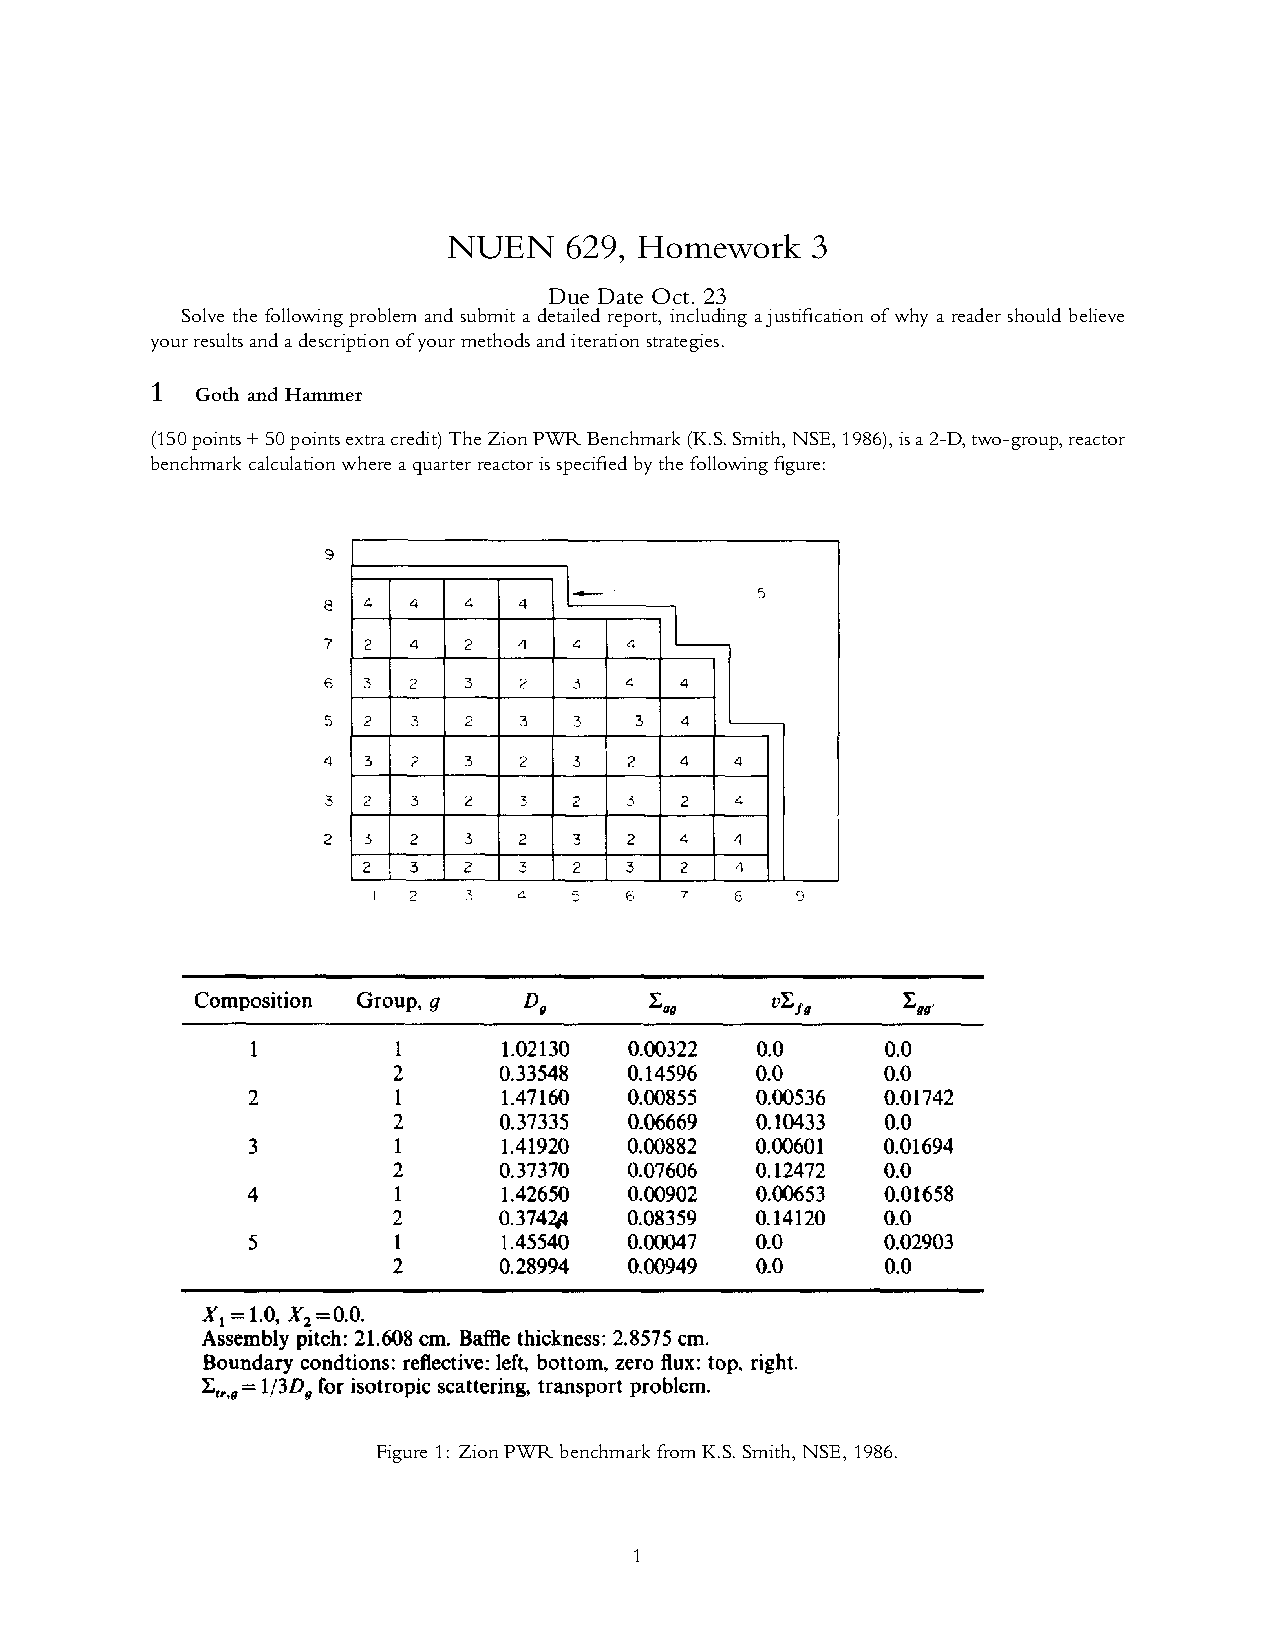
\includepdf{Homework3.pdf}

\begin{solnum}{1-1}
    
The 2D lattice input code provided in lab was modified to generate the input for the
first
benchmark problem.  Because the
provided code assumes a uniform mesh size, approximations must be made to resolve the
baffle in the geometry.  I have assumed that if a particular cells center lies with
in the region of the baffle, then that cell has the baffle material properties.  Also, I have assumed that the assemblies near the reflecting
boundary are full assemblies, rather than half assemblies. To match the edges of the
assembly exactly, I used numbers of cells in the $x$ and $y$ direction that are
factors of 9.  It is noted that this will cause a jump in convergence of the solution
in terms of mesh size, caused at points where the cell widths are small enough that
an additional baffle  cell can be inserted.  

The assembly power is averaged over each
cell in a 9x9 grid over the quarter reactor, weighted by $\nu \Sigma_f$ in each
group.  Since we do not know $\Sigma_f$ individually this is not exact since $\nu$ is
larger for the fast group, generally.  Since we are normalizing, this is not a great
error, and produces a zero assembly power in the water regions as desired.

A convergence table versus mesh size as a function of the number of cells is given
below.  It appears that the solution is convergent above 3969 cells and that it
would reach a tolerance of 1 pcm around 12,000 cells, noting that there is some
variablity due to the baffle approximations.  The time to solution at 8100
cells is 1600 seconds. 

\begin{table}
    \centering
    \caption{Convergence table for finite difference method versus number of mesh
    cells.}
\begin{tabular}{ccc} \hline
81   & 1.2786193689  &  -- \\ 
324       & 1.27611471632   & 0.00250465258332 \\
729       & 1.27609454035   & 2.01759703702e-05 \\
1296      & 1.27623214214   & 0.00013760179336  \\ 
2025 & 1.27586573839 & 0.000290925744068  \\
2916 & 1.27563942334 & 0.000177413023663  \\
3969 & 1.27549513858 & 0.000113120586226  \\
5184 & 1.27540107208 & 7.37544516677e-05  \\
6561 & 1.27533957529 & 4.82199314754e-05  \\ \hline
8100 & 1.27530010292 & 3.09514302439e05   \\ \hline
    \end{tabular}
\end{table}

\begin{figure}
    \centering
    \caption{Material ID's for Problem 1. There is a slight error due to how pcolor
    interpolates linear values at cell centers, so the entire picture is shifted}
    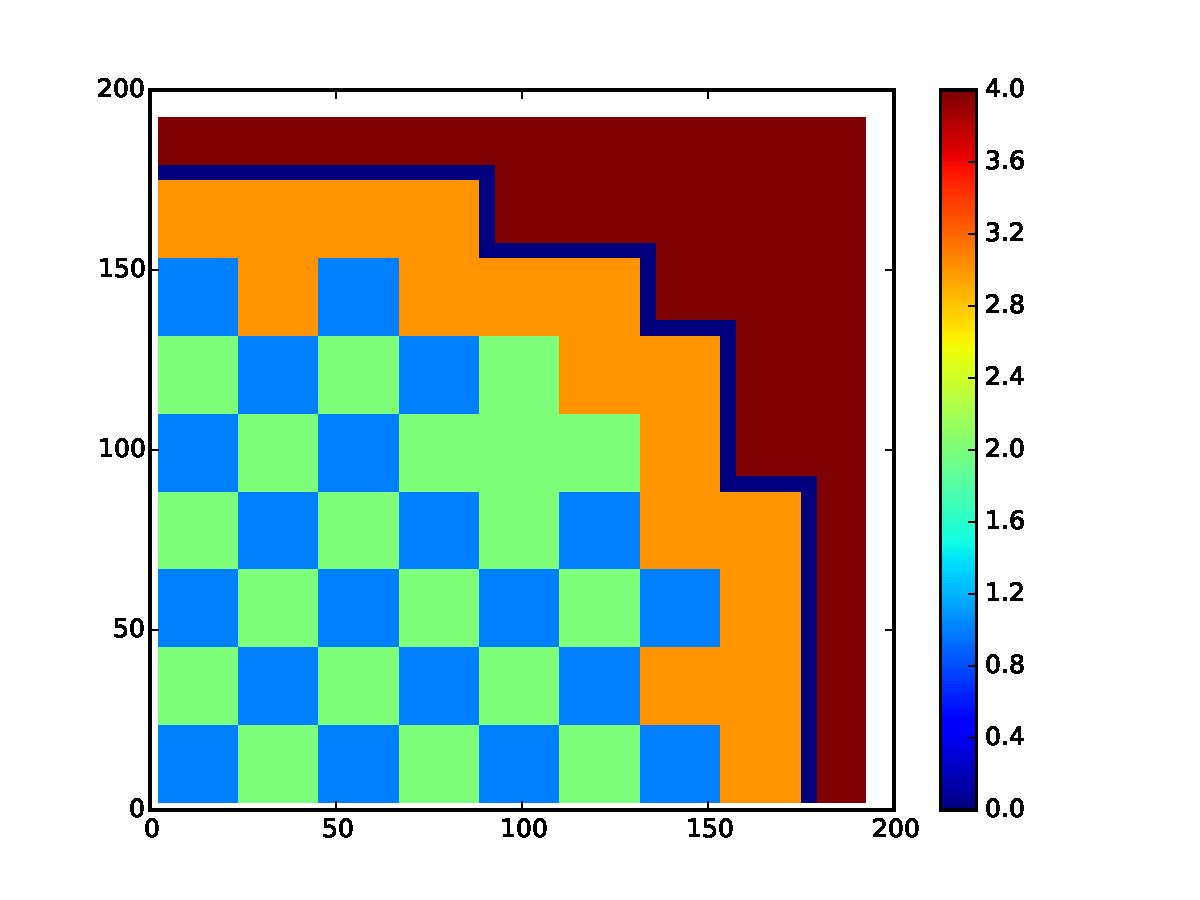
\includegraphics[width=0.5\textwidth]{geometry.pdf}
\end{figure}

\begin{figure}
    \centering
    \caption{Normalized group 1 fluxes for finite difference solution}
    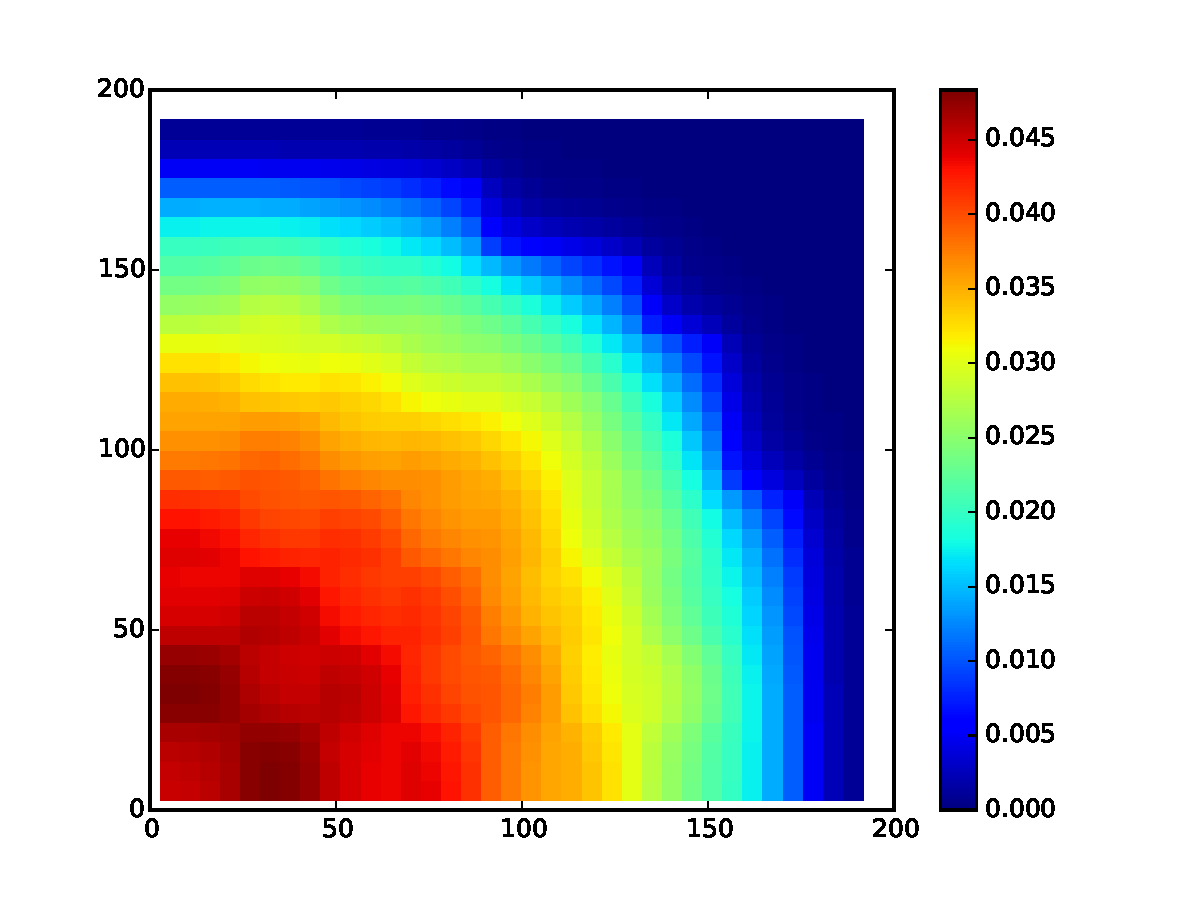
\includegraphics[width=0.5\textwidth]{prob1_diff_g1.pdf}
\end{figure}

\begin{figure}
    \centering
    \caption{Normalized group 2 fluxes for finite difference solution}
    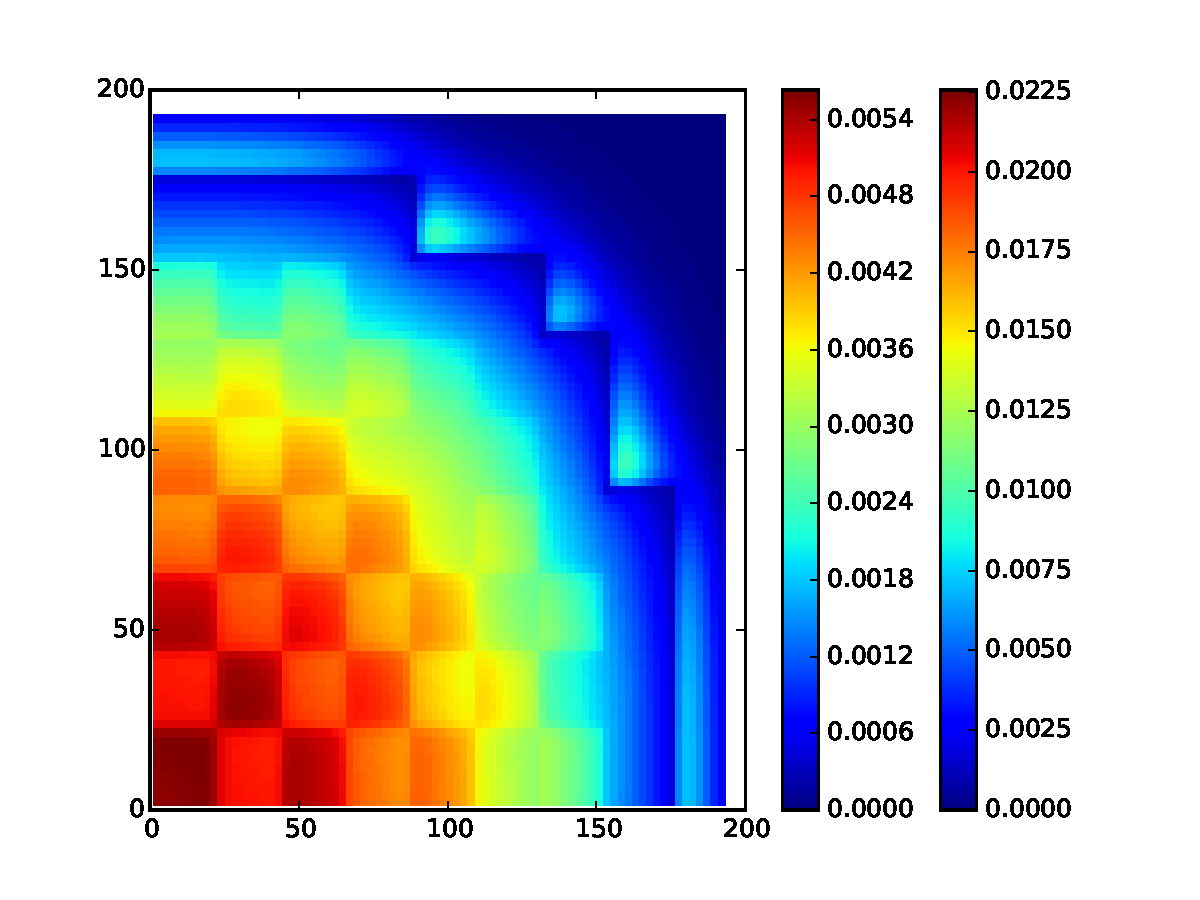
\includegraphics[width=0.5\textwidth]{prob1_diff_g2.pdf}
\end{figure}

\begin{figure}
    \centering
    \caption{Assembly (assuming 9x9 grid) averaged powers for problem 1, normalized
    to the max assembly power, solved using finite differences. Note: there is a slight error in the way pcolor is interpolating values.}
    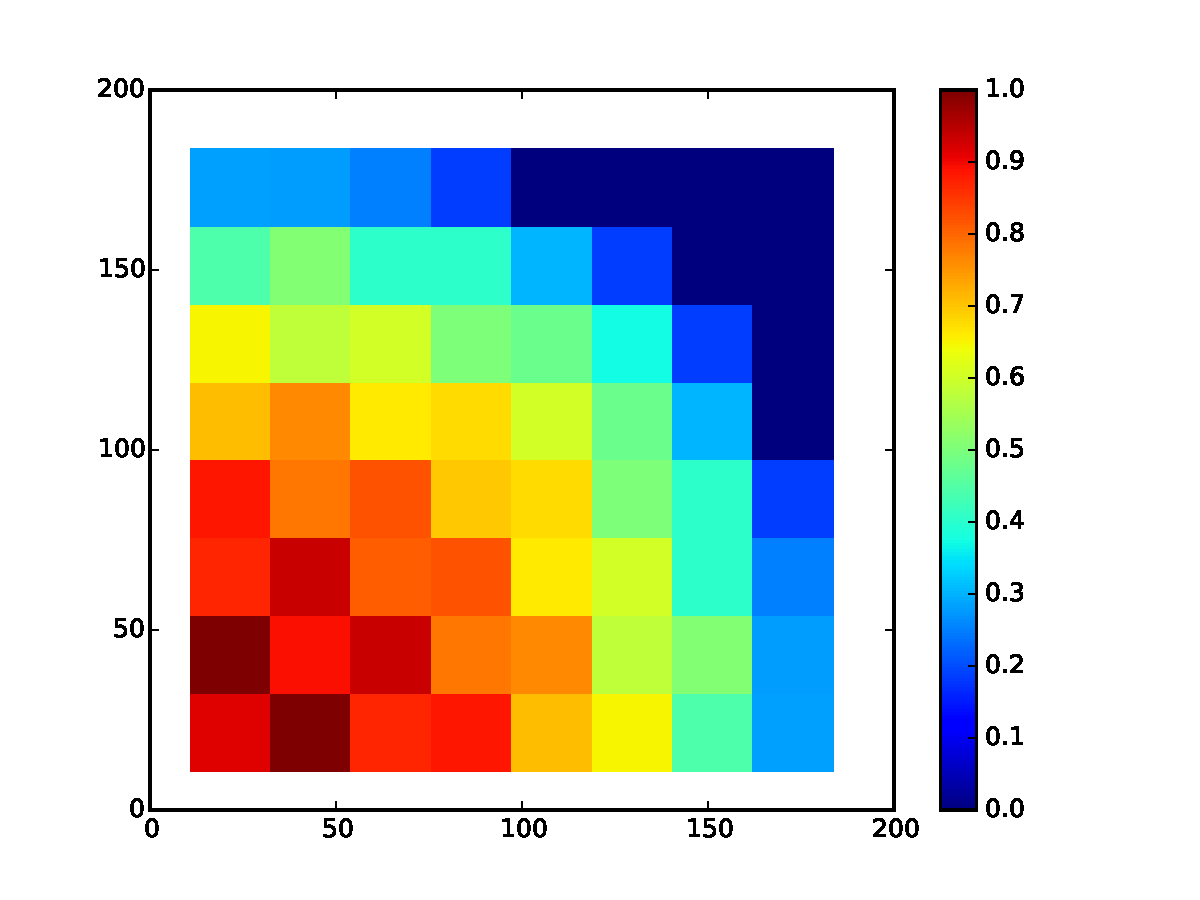
\includegraphics[width=0.5\textwidth]{powers_diff.pdf}
\end{figure}

\end{solnum}
\clearpage

\begin{solnum}{1-2}

The provided $k$ code and nodal code were modified to solve $k$ problems using the
nodal method.  The outer iterations were essentailly unmodified, with only the 2D
steady fixed-source solve modified.
The provided algorithms for the nodal method in class had to be modified to produce a
stable algorithm. Although it
is not the most efficient, the method is modified to use internal solution for
computing the transverse total currents.  For example, for the nodal solve in the $x$
direction, the $y$ transverse leakage term becomes
\begin{equation*}
  L_y,ij(x) = \frac{1}{h_y}\left(\overline{J}^y_{ij}(x_i,y_j+h_y/2) -
  \overline{J}^y_{ij}(x_i,y_j-h_y/2) \right)
\end{equation*}
where, for simplicity, the transverse current has also been assumed as a piecewise
constant spatially along the direction of the nodal solve, and the $L_x$ and $L_y$
terms in their respective solves are lagged for the entire sweeps (Jacobi
iteration). Because I have used Marshak or reflective boundary conditions, using the
same equation for boundary cells also strictly enforces the boundary condition.

The iteration would
likely be more efficient if the outward partial currents from the cell were used for
the transverse leakages, with the inflowing currents coming from adjacent cells, however I did not test this approach
for stability.  If we use the total current from adjacent cells for the leakage
terms, then the iteration is not stable.  I believe this is due to
the fact that the transverse 
current (which was computed by the previous nodal solve in the transverse direction)
was computed using a lagged inflow to the adjacent cell.  We are now using that
lagged inflow as the transverse outflow within our cell.  Thus, the transverse outflow to the
cell of interest is 2 iterations behind, and this seems to be too inaccurate for
stability.  

Due to time constraints and because the nodal iteration was very slow, I did not
attempt to converge $\keff$ to 1.E-05.  A plot of the group fluxes and assembly powers are
given below for the case of 729 cells.  For this case $\keff$ was found to be
1.273.  This is in agreement with the finite difference solution, noting that the baffle is extra
large since there is only 2 cells in each assembly in this case.  With a loose tolerance of 1.E-04 on all iteration loops, this solve took
990 seconds, so this method is very slow without the CMFD acceleration. The thermal flux appears to not be fully converged
\begin{figure}
    \centering
    \caption{Normalized group 1 fluxes for nodal method solution with 729 cells}
    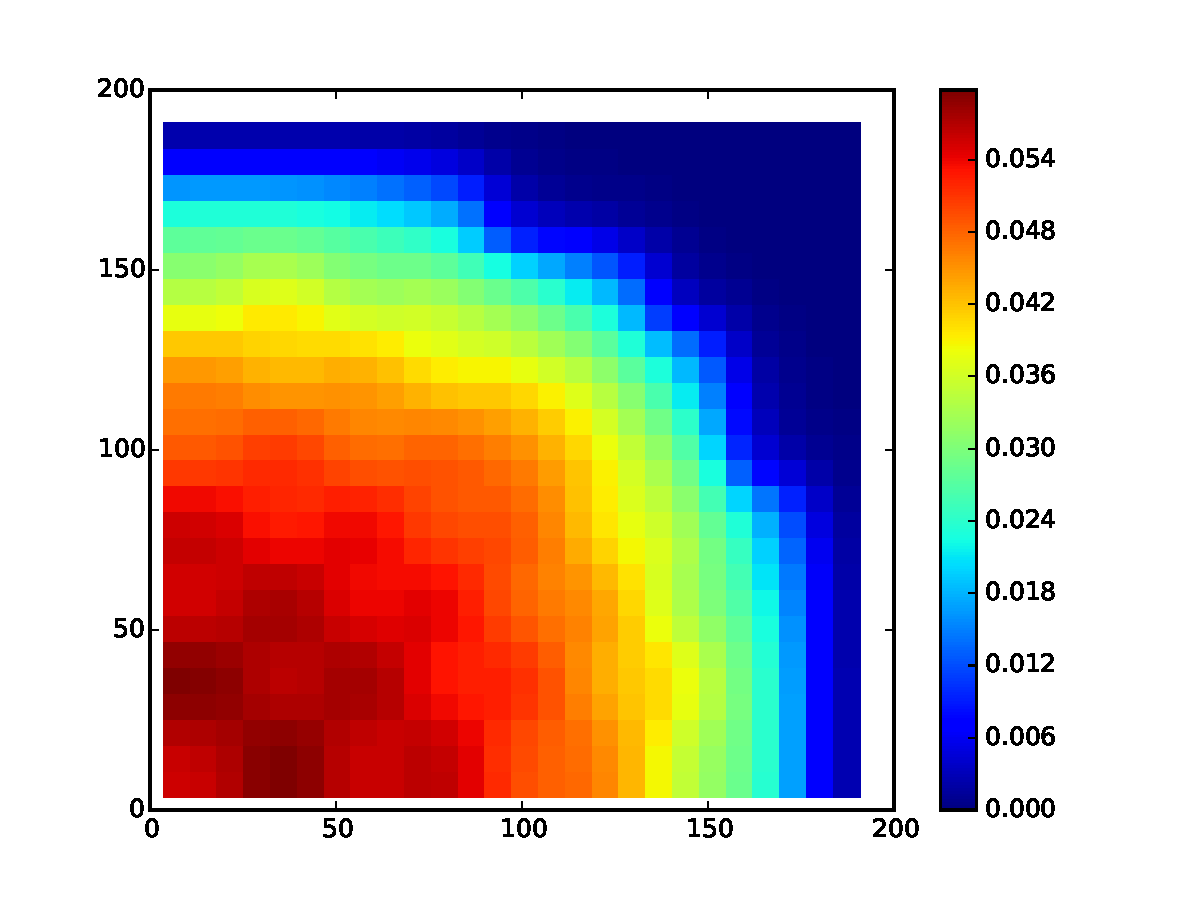
\includegraphics[width=0.5\textwidth]{prob1_g1_nodal.pdf}
\end{figure}

\begin{figure}
    \centering
    \caption{Normalized group 2 fluxes for nodal method with 729 cells}
    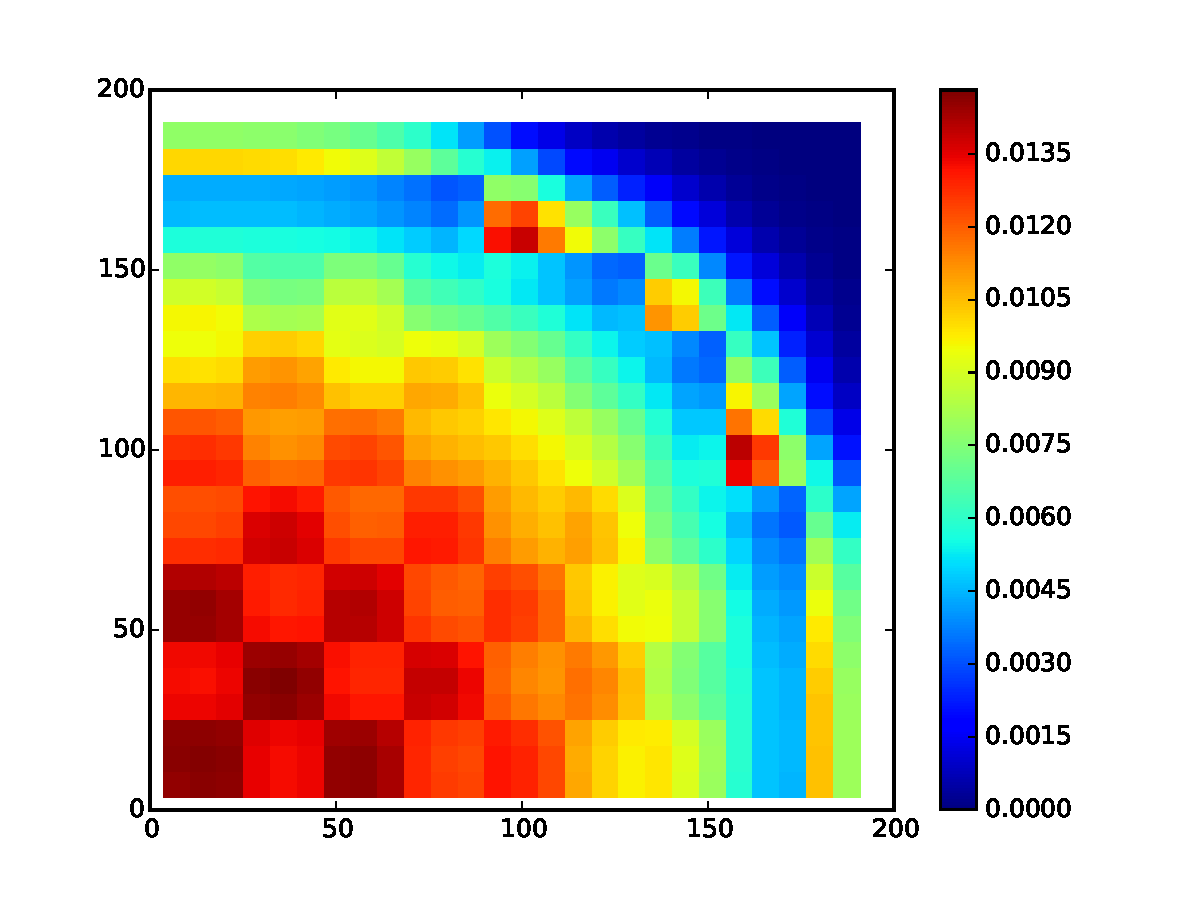
\includegraphics[width=0.5\textwidth]{prob1_g2_nodal.pdf}
\end{figure}

\begin{figure}
    \centering
    \caption{Assembly (assuming 9x9 grid) averaged powers for problem 1, normalized
    to the max assembly power, solved using nodal method. Same issues with pcolor interpolating strangely, the edge of boxes are actualy the center of assemblies}
    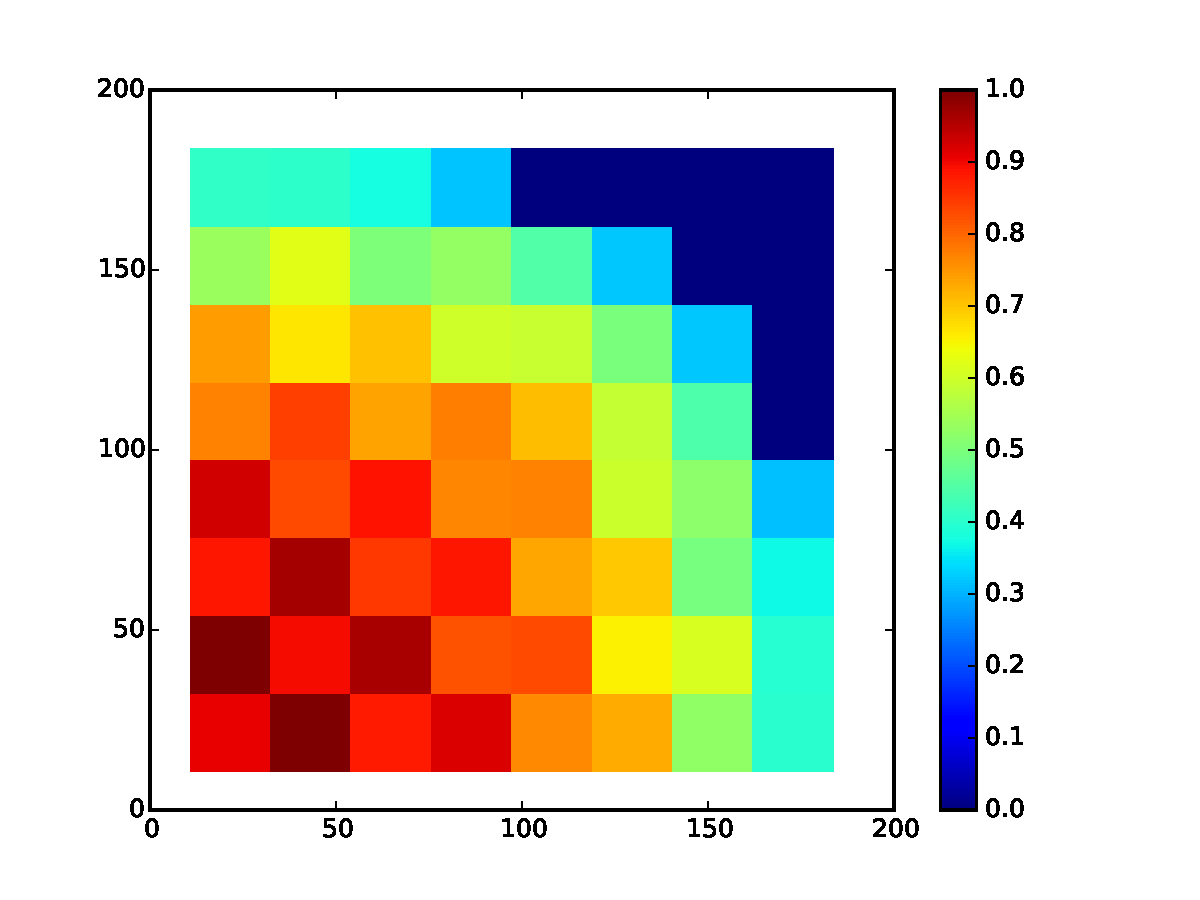
\includegraphics[width=0.5\textwidth]{powers_nodal.pdf}
\end{figure}



\end{solnum}

\clearpage

\begin{solnum}{1-3}

Because the nodal code is very slow, the finite difference code was used to determine
the critical reactor height. The secant method was used to determine the critical
height to a relative tolerance in $\keff$ of 1.E-05, taking 11 iterations on $H$
from an initial educated guess of $50$ cm.  A mesh was used with 729 elements. The
critical height was found to be  $46.85$ cm, producing a $\keff$ of 0.999996. This
is a reasonable number since the 2D reactor had a relatively high $\keff$ of
$\sim$1.27.
\end{solnum}

\clearpage

\clearpage
\subsubsection*{Code}
\lstinputlisting[basicstyle=\scriptsize]{code.py}

\end{document}

